\documentclass[12pt,fleqn]{article}\usepackage{../../common}
\begin{document}
Ders 11

Bu ders oldukça teorik olacak ama içindeki fikirler bu derste öğretilen en
önemli fikirlerin arasında. Şu denklemi hatırlarsak

$$ y'' + p(x)y' + q(x)y = 0 $$

Bu denklemin çözüm yöntemi iki tane bağımsız $y_1$ ve $y_2$ bulmaktan
geçiyordu. Bağımsızlığın tanımı mesela $y_2$'nin $y_1$'in ``katı''
olmaması, yani bir çözümü tamsayı bir sabitle çarpınca diğerini elde
edememeliyiz. Yani $y_2 \ne cy_1$, ve $y_1 \ne c'y_2$, ve $y_1 = 0$ ise
$y_2$ sıfır olmamalı. 

Üsttekileri belirtmemizin sebebi neydi? Ki böylece ODE'nin tüm çözümlerinin
$y_1$ ve $y_2$'nin bir lineer kombinasyonu olduğunu söyleyebilmek, yani

$$ y = c_1 y_1 + c_2 y_2 $$

Bu derste cevaplandıracağımız soru şu: Niye? 

Soru 1: Niye $c_1 y_1 + c_2 y_2$'in hepsi bir çözümdür?

Bu soruyu bu dersteki öğrenciler cevaplayabilir herhalde, fakat temiz, öz,
zarif (elegant) bir şekilde cevaplayabilmek önemli olan ve aslında bu
dersin de konusu. Bu cevabı öz, temiz bir şekilde veremezsek, daha ileride
daha çetrefil işleri halledemeyiz. 

Birinci soru lineer kombinasyonların niye çözüm olduklarını cevaplayacak,
fakat ``tüm'' çözümlerin onlar olduğunu daha zor olan 2. sorunun cevabı
belirleyecek.

Soru 2: Niye tüm çözümler bunlardır?

Birinci sorunun cevabı üst üste eklenebilmek (superposition) prensibi sayesinde
cevaplanacak, ki bu prensip lineer kombinasyon argümanıyla aynı şey. Ek bir not
bu prensibin ODE hangi dereceden olursa olsun (yani 2 olduğu gibi, 3, 4,
vs. bile olabilir, form değişmediği sürece derece artabilir) prensibin geçerli
olmasıdır.

Bu ispatı yapmanın temiz yöntemlerinden biri, azıcık yol dışına çıkıp
(detour), lineer operatörlerden bahsetmektir. Bu operatörleri dersimizin
geri kalanında sürekli kullanacağız, onları iyice tanımamız iyi olur. 

Amacım üst üste eklenebilme prensibinin ispatı, oraya gelirken, değişik
yerlere girip çıkacağız. Ana formu tekrar yazalım. 

$$ y'' + p(x)y' + q(x)y = 0 $$

Şimdi bu formu türev alma operatörünü kullanarak tekrar yazacağım. Operatör
$D$, bir kere türev al demektir, $D^2$ iki kere türev al demektir. O zaman

$$ D^2y + pDy + qy = 0  $$

$y$'yi dışarı çekelim

$$ (D^2 + pD + q)y = 0  $$

Burada dikkat: insanlar yukarıdaki ibareyi ``parantez içinde bir şeyler
{\em çarpı} y'' diye okumaya meyilli oluyor, bu doğru değil. Böyle bir ima
var gibi ama gerçekte olan bu değil, çünkü D operatörü y ``üzerinde'' işlem
yapan bir operatör. Aslında üsttekini yaparken amacım şuydu, parantez
içindeki her şeyi başlına başına tek bir operatör haline çevirmek, ki bu
operatöre $L$ adı verelim

$$ \underbrace{(D^2 + pD + q)}_{L}y = 0  $$

O zaman geriye 

$$ Ly = 0 $$

kalır. Formel olarak $L$'nin tanımı üsttekidir, onu zihnimizde bir kutu
olarak ta canlandırabiliriz, kutuya bir fonksiyon giriyor, dışarı başka bir
fonksiyon çıkıyor.

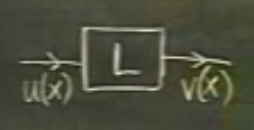
\includegraphics[height=3cm]{11_1.png}

Daha da detaylandırmak gerekirse, sayılar için fonksiyonlar neyse,
fonksiyonlar için operatörler o'dur. Bir fonksiyona sayı girer, dışarı sayı
çıkar, bir operatöre ise fonksiyon girer, bu fonksiyon değişime uğrayıp
dışarı başka fonksiyon olarak çıkar. Türev alma operatörü en basit
örneklerden biridir, mesela $x^2$ fonksiyonu türev operatörü $D$'ye girerse,
dışarıya yeni bir fonksiyon $2x$ çıkar.

ODE'ye dönersek, üstteki ODE'yi çözmek demek $L$ kutusundan sıfır çıktığını
düşünmek ve bunun olması için kutuya ne girdiğini bulmaya çalışmak. Bir
ODE'yi çözmek, o zaman, bir tersine çevirme (inverse) problemidir. Tabii
ters yönde gitmek ileri yönde gitmekten daha zordur. 

Bu operatörün lineer olduğunu hatırlayalım. Bu, operatör fonksiyonlarla
iş gördüğü zaman belli özellikler gösterir. 

$$ L(u_1 + u_2) = L(u_1) + L(u_2) $$

$$  L(cu) = cL(u)$$

ki $c$ bir sabit, $u$, $u_1$ ve $u_2$ fonksiyonlardır. 

Üstteki iki ifade lineerliğin iki kuralıdır. Bu kurallar normal
fonksiyonlar için de geçerlidir bu arada. 

Örnek? $D$ operatörü lineer bir operatördür. Çünkü, mesela

$$ (u_1 + u_2)' = u_1' + u_2' $$

$$ (cu)' = cu' $$

Bu Calculus dersinden bildiğimiz bir şey. Yani en temel Calculus'tan
beri bildiğimiz üstteki kurallar aslında $D$ operatörünün lineer bir
operatör olduğunun da göstergesidir.

Not: Ya peki çarpma? O da bir şekilde duruma dahil mi? Onun da kullanıldığı
bazı durumlar var ama lineerlik bağlamında konumuzun dışında.

Neyse, tüm bu kuralları üst üste eklenebilme prensibini ispatlayabilmek
için ortaya koyduk, şimdi ispatın kendisine gelelim. 

Teori

ODE'miz şöyle:

$$ Ly = 0 $$

Eğer $y_1$ ve $y_2$ çözüm ise alttaki de bir çözümdür.

$$ y = c_1 y_1 + c_2 y_2 $$

İspat

$L$ operatörünü üstteki kombinasyona uygulayalım:

$$ L(c_1 y_1 + c_2 y_2) = L(c_1 y_1) + L(c_2 y_2)$$

$$ = c_1L(y_1) + c_2L(y_2)$$

Şimdi yapmaya çalıştığım bunu sıfır olduğunu göstermek. Eğer $y_1$ bir
çözüm ise o zaman $Ly=0$'dan hareketle $L(y_1)$'in sıfır olması
gerekir. Aynı şekilde $L(y_2) = 0$.

$$ = c_1 \cdot 0 + c_2 \cdot 0 = 0 $$

İspat tamamlandı. Bu argümanı ODE'nin orijinal formunu kullanarak ta
yapabilirdik tabii, ama o zaman değişkenleri yerine koyup cebirsel gruplama
yapacak, bir sürü işlem içine girecektik. Bu bize sonucu verecekti, ama ispatın
niye böyle sonuç verdiğini açık bir şekilde söylemeyecekti. İspat başarılı oldu
çünkü $L$ bir lineer operatördü.

Şimdi daha zor olan ikinci soruya gelelim. Bu soruyu cevaplayacağız, ama
bir yan yola girerek, cevabı ``başlangıç değer problemini çözme'' açısından
anlamaya uğraşacağız, başlangıç değerlerini formüle uydurarak (fitting) bir
yere gelmeye çabalayacağız. 

Teori

Tüm lineer kombinasyonları bir küme olarak düşünelim, 

$$ \bigg\{ c_1y_1 + c_2y_2 \bigg\} $$

Bana hangi başlangıç değerini verirsen verin, bu küme içinde ona uygun bir
$c_1$ ve $c_2$ bulabilirim. 

İspat

Bu ispatı yaparken şimdiye kadar ODE çözerken ödevlerde geliştirdiğimiz
başlangıç değerlerini kullanıp sabitleri hesaplama becerisinden
faydalanacağız, ama sayılar yerine semboller kullanacağız. Diyelim ki 

$$ y(x_0) = a $$

$$ y(x_0) = b $$

Yerine koyarsak

$$ y = c_1y_1 + c_2y_2 $$

$$ y' =  c_1y_1' + c_2y_2'$$

$x=x_0$'i yerine koyalım

$$ y = c_1y_1(x_0) + c_2y_2(x_0) = a$$

$$ y' =  c_1y_1'(x_0) + c_2y_2'(x_0) = b$$

Ödev problemlerinde $y_1$ ve $y_2$ somut fonksiyonlar oluyordu, $e^x$ gibi
mesela. Burada sadece onun yerine sembolik değerler kullanıyorum. 

Şimdi üstteki iki denkleme bakalım. Bu bir beraber çözülecek (simultaneous)
lineer denklem sistemi değil midir? Çözülecek, bulunacak değişkenler
hangileri? $c_1$ ve $c_2$. Buna tam alışkın değiliz, genellikle çözülecek
değişkenler terimlerin önünde değil arkasında olur, üstelik $c_1$ ve $c_2$
şimdiye kadar hep ``sabit'' olarak etiketlediğimiz şeyler, ama biraz daha
düşünürsek ve geri kalan arap saçı gibi terimlere dikkatlice bakarsak
lineer sistemi görebiliriz. Bu sistemde değişkenler $c_1$ ve $c_2$. 

Peki şimdi şu soruyu soralım. Üstteki sistemin ne zaman bir çözümü vardır?
Sistem her zaman çözülemeyebilir. Cevap: Eğer katsayı matrisinin tersi
alınabiliyor ise (invertible), yani matrisin determinantı sıfır haricinde
bir değer olmalı. 

$$ 
\left|\begin{array}{rr}
y_1 & y_2 \\
y_1' & y_2'
\end{array}\right|_{x_0}
\ne 0
$$

Determinant işareti $|$'nin alt köşesindeki $x_0$, matris içindeki tüm
fonksiyonların $x_0$ verilerek elde edilen sonuçlarını kullanmamız
gerektiğini söylüyor.  

Üstteki determinant önemli bir determinant, ve bir ismi var:
Wronskian. Sembolik kullanımi ise şöyle: $W(y_1, y_2)$. Hepsini bir arada
belirtirsek, 

$$ W(y_1, y_2) = 
\left|\begin{array}{rr}
y_1 & y_2 \\
y_1' & y_2'
\end{array}\right|
 $$

Wronskian'ı ona geçilen iki fonksiyonu biliyorsak hesaplayabiliriz, ama
$W$, $y_1$ ve $y_2$'nin fonksiyonu değil. Wronskian $x$'in bir fonksiyonu
aslında. 

Wronskian'ın sıfır olmama durumunu nasıl ispatlarız? Diyelim ki $y_2$ ve
$y_1$ birbirine bağımlı (dependent), yani $y_2 = cy_1$. Bunun böyle
olmadığını biliyoruz çünkü ODE'nin farklı çözümleri var. Ama olduğunu
düşünelim, ve üstteki determinanta bakalım, $y_2 = cy_1$ olması ne
demektir?  $y_2' = cy_1'$ şartının da geçerli olması demektir. Ve bu şart
gerçekleşirse, o zaman Wronskian, her $x$ değeri için, her zaman,
kesinlikle sıfır olacaktır, çünkü artık iki kolon tamamen birbirinin katı
haline gelmiştir.

Ödev sorularında öğrencinin ispatlamasını istediğimiz teori bu. 

Teori

Eğer $y_1$ ve $y_2$ ODE'mizin çözümü ise, o zaman sadece iki seçenekten
biri doğru olabilir. Ya her $x$ değeri için $W(y_1,y_2) = 0$ (aslında her
$x$ değeri için sözü fazlalık, çünkü Wronskian tanımı zaten o ifadeyi
kapsıyor, ama bu bir giriş dersi olduğu için tekrarlıyoruz), ya da
Wronskian hiçbir zaman sıfır değil.

Şimdi, bir parantez daha açıyoruz. Bu ikinci parantez de kapanınca, üstteki
``2. sorunun'' cevabını vermek için elimizde tüm gerekli araçlar olacak. 

Yukarıda ODE çözümünün tüm çözümlerinin şurada olduğunu belirtmiştik

$$ \bigg\{ c_1y_1 + c_2y_2 \bigg\} $$

Önemli nokta şu ki, $y_1$ ve $y_2$ öyle ``özel'', ``kutsal'' çözümler
değiller. Şunu da söyleyebilirdik ve üstteki ifade ile aynı şey olurdu

$$ \bigg\{ c_1'u_1 + c_2'u_2 \bigg\} $$

ki $u_1$ ve $u_2$ herhangi başka bir lineer olarak bağımsız çözümler. 

Bunu niye söyledik? $y_1$ ve $y_2$ genelde denklemi çözdüğümüz zaman elde
ettiğimiz kolay çözümlerdir, mesela $e^x$, $e^2x$, $\cos(x)$,
vs. türünde. Çözümü bu tür öğeleri kullanarak yazmak bir yöntem tabii,
fakat tek yöntem değil. Bazı ODE'ler için ``normalize edilmiş çözümler''
bulmak daha iyi. 

Normalize edilmiş çözümler belli bazı özel başlangıç şartlarını tatmin eden
çözümlerdir. Eğer $Y_1$ ve $Y_2$'yi normalize edilmiş çözümler olarak kabul
edersek, bu şartlar

$$ Y_1(0) = 1, \quad  Y_2(0) = 0  $$

$$ Y_1'(0) = 0, \quad  Y_2'(0) = 1 $$

Örnek 

$$ y'' + y = 0 $$

Standart çözümler $y_1 = \cos(x)$, $y_2 = \sin(x)$. $y_1$'in 0'daki değeri
nedir? 1. $y_1'$'in sıfırdaki değeri nedir? 0. Demek ki $y_1$ normalize
edilmiş, yani $Y_1$. $y_2$ aynı şekilde $Y_2$ olur. 

Not: Normalize çözümleri çoğunlukla bir bakışta bu kadar kolay göremiyoruz
tabii ki. 

Örnek 

$$ y'' - y = 0 $$

Karakteristik denklemler 1, ve -1, o zaman çözüm $y_1 = e^x$ ve $y_2 =
e^{-x}$. 

Genel çözüm 

$$ y = c_1 e^x + c_2 e^{-x} $$

Buradan normalize çözümleri, mesela $Y_1$, nasıl buluruz? Başlangıç
şartlarını yerine getirerek. Bu arada $y'$

$$ y' = c_1 e^x - c_2 e^{-x} $$

Şartları koyalım. $y_1(0)$

$$ c_1 + c_2 = 1 $$

$y_1'(0)$

$$ c_1 - c_2 = 0 $$

Bu bir denklem sistemi yarattı, o zaman $c_1 = c_2 = 1/2$. O zaman 

$$ Y_1 = \frac{e^x + e^{-x}}{2} $$

$Y_2$'yi benzer şekilde buluruz, hesapları yaptıktan sonra sonuç

$$ Y_2 = \frac{e^x - e^{-x}}{2} $$

çıkacaktır. Yani örnek ODE'miz için bu iki çözüm normalize edilmiş
çözümlerdir. Bu çözümler asıl çözümlerden ``daha iyi'', çünkü başlangıç
şartları daha ``güzel''. Çözüme ve türevini sıfır noktasında hesaplayınca
bunu görüyoruz, sonuç ya 0 ya da 1 geliyor. Temiz. Bu arada bu örnekte elde
ettiğimiz $Y_1$, $\cosh(x)$ (hiperbolik kosinüs) ve $Y_2$, $\sinh(x)$
(hiperbolik sinüs) olarak bilinir. 

Mühendisler normalize çözümleri çok severler, çünkü eğer $Y_1$ ve $Y_2$
sıfırda normalize edilmişse, o zaman başlangıç değer problemi, yani bizim
klasik ODE'miz artı

$$ y(0) = y_0 $$

$$ y'(0) = y_0' $$

denkleminin çözümü şöyledir

$$ y = y_0 Y_1 + y_0' Y_2 $$

Diğer bir deyişle, eğer bir denklemin normalize çözümlerini bulmuşsak /
biliyorsak, genel çözüm için başlangıç şartlarını {\em olduğu gibi} alıp
genel çözümü yaratmak için kullanabiliriz. 

Üstteki $y$'nin doğru olup olmadığı kontrol edilebilir. Mesela $y(0)$
nedir? O noktada $Y_1(0)=1$, $Y_2(0)=0$ olduğuna göre  $y(0)=y_0$ elde
ederiz, ki bu üstteki başlangıç şartları ile uyar. Geri kalanını siz
kontrol edebilirsiniz. 

Böylece ikinci parantezi kapattık. Artık ``büyük teori'' için gereken her
şey var.

Mevcudiyet ve Özgünlük Teorisi (Existence and Uniqueness Theorem)

Standart ODE

$$ y'' + py' + qy = 0 $$

öyle ki $p$ ve $q$ her $x$ için sürekli fonksiyonlar (``iyi'' fonksiyonlar
yani, katsayılar hiçbir noktada patlamıyor). 

O zaman, bu teoriye göre, verilen başlangıç şartları

$$ y(0) = A $$

$$ y'(0) = B $$

uyumlu bir çözümü, ve sadece bir tane çözüm vardır. 

Bir çözüm olması teorinin ``mevcudiyet'' tarafı, o çözümün tek mümkün çözüm
olması teorinin özgünlük tarafı. 

İddia ediyorum ki 

$$ \bigg\{ c_1Y_1 + c_2Y_2 \bigg\} $$

kümesi tüm çözümleri içeriyor. 

İspat

Verilen herhangi (arbitrary) bir çözüm $u(x)$, ki

$$ u(0) = u_0 $$

$$ u'(0) = u_0' $$

alınıp şu şekilde kullanılınca

$$ u_0 Y_1 +  u_0'Y_2 $$

bu ifade başlangıç şartlarıyla uyumlu olur. 

Ekler

Dersler 9-11 içeriğinde ikinci derece lineer diferansiyel denklemin eğer iki
çözümü varsa onların lineer birleşiminin yeni bir çözüm olacağını aktardık,
başlangıç şartlarını dahil edince bir çözüm bulunacağını gördük. Wronskian bu
bağlamda iki çözümün ``birleştirilebilir'' olup olmadığını kontrol ediyordu.
Fakat bulduğumuz çözümün özgün (unique) olup olmadığını hala bilmiyoruz, en
azından şu anda kadar onun için teorik bir ispat görmedik.

$$
ay'' + by' + cy = 0
$$

Mesela üstteki gibi sabit katsayılı ikinci derece denklem çözümü için $e^{rt}$
seçimi yaptık, bunu bir bilgili tahmin (ansatz) olarak gerçekleştirdik, fakat bu
seçimin temeli nedir? Seçilen fonksiyon özgün çözüm müdür?

Sezgisel olarak $\exp$ bazlı bir çözüm işleyeceğini bilebilirdik, çünkü birinci
derece baz lineer diferansiyel denklemin çözümü bir $\exp$ içerir. Sezgisel
tahmin şöyle devam eder, ikinci derece lineer denklemi birinci derece
diferansiyel denklem {\em sistemine} çevirebileceğimize göre $\exp$ fonksiyonu
seçimi normaldir.

Ya da, şöyle düşünürdük, üstteki formül bize şunu çıtlatıyor sanki, ikinci
türev, birinci ve sıfırıncı türevlerin lineer kombinasyonu olarak temsil
ediliyor olabilmeli [2, sf. 158] .. Bu bizi yine $y = e^{rt}$ şeklinde bir
formüle itebildi, çünkü $e^{rt}$'nin türevleri bir sabit çarpı $e^{rt}$'nin
kendisi olacaktır.

Fakat bize akıllı tahminlerin ötesinde çözümün varlığını ve özgünlüğünü
kanıtlayan net, kesin (rigourous) bir ispat gerekiyor. Önce en temel başlangıç
değer problemi (initial value problem -IVP-) ile başlayalım.

$$
y' = f(x,y), \quad y(x_0) = y_0
\mlabel{1}
$$

Üstteki IVP yerine alttaki gibi, ona eşit bir entegral formülü geçirebiliriz,

$$
y(x) = y_0 + \int_{x_0}^{x} f[t, y(t)] \ud t
\mlabel{2}
$$

Bu formulu (1)'in entegralini alarak elde ettik, bu bariz, baslangic sartini
$y_0$ terimi uzerinden dahil ettik.

Simdi (2)'yi ozyineli bir sekilde cozmeye ugrasacagiz. 3














[devam edecek]

Kaynaklar

[1] Boyce, {\em Elementary Differential Equations Boundary Value Problems}

[2] Nagle, {\em Fundamentals of Differential Equations and Boundary Value Problems}

[3] Simmons, {\em Differential Equations With Applications and Historical Notes}

\end{document}

